% This is text associated with the open textbook "Open Electromagnetics"
% See immediately below for author, date
% This work is licensed under the Creative Commons Attribution-ShareAlike 4.0 International License. (CC BY-SA 4.0) 
% To view a copy of the license, visit http://creativecommons.org/licenses/by-sa/4.0/

%ORB TITLE Electric Potential Field Due to Point Charges
%ORB AUTHOR 0        # S.W. Ellingson, Virginia Tech (ellingson@vt.edu)
%ORB DATE 20180806   # yyyymmdd
%ORB ABSTRACT Electric Potential due to Point Charges

\label{m0064_V_due_to_Point_Charges} % <-- Must match name of this file and module directory name.  Don't mess with this!

The electric field intensity due to a point charge $q$ at the origin is
(see Section~\ref{m0102_Coulombs_Law} or \ref{m0014_Gauss_Law_Integral_Form}) 
%
\begin{equation}   
{\bf E}  = \hat{\bf r}\frac{q}{4\pi\epsilon r^2}
\label{eEPPCE}
\end{equation}
%
In Sections~\ref{m0061_Force_Energy_and_Potential_Difference} and \ref{m0062_Independence_of_Path}, it was determined that the potential difference measured from position ${\bf r}_1$ to position ${\bf r}_2$ is
%
\begin{equation}
V_{21} = - \int_{{\bf r}_1}^{{\bf r}_2} {\bf E} \cdot d{\bf l}
\label{m0064_eV12}
\end{equation}

This method for calculating potential difference is often a bit awkward.  
To see why, consider an example from circuit theory, shown in Figure~\ref{m0064_fResistor}.
In this example, consisting of a single resistor and a ground node, we've identified four quantities:
%
\begin{itemize}
\item The resistance $R$
\item The current $I$ through the resistor
\item The node voltage $V_1$, which is the potential difference measured from ground to the left side of the resistor 
\item The node voltage $V_2$, which is the potential difference measured from ground to the right side of the resistor
\end{itemize}
%
Let's say we wish to calculate the potential difference $V_{21}$ across the resistor.
There are two ways this can be done:
%
\begin{itemize}
\item $V_{21}=-IR$  
\item $V_{21}=V_2-V_1$
\end{itemize}
%
The advantage of the second method is that it is not necessary to know $I$, $R$, or indeed anything about what is happening between the nodes; it is only necessary to know the node voltages.
The point is that it is often convenient to have a common \emph{datum} 
\index{datum}
-- in this example, ground 
\index{ground}
-- with respect to which the potential differences at all other locations of interest can be defined.  When we have this, calculating potential differences reduced to simply subtracting predetermined node potentials.
%
\begin{figure}
\begin{center}
\pdftooltip{{  % note double braces
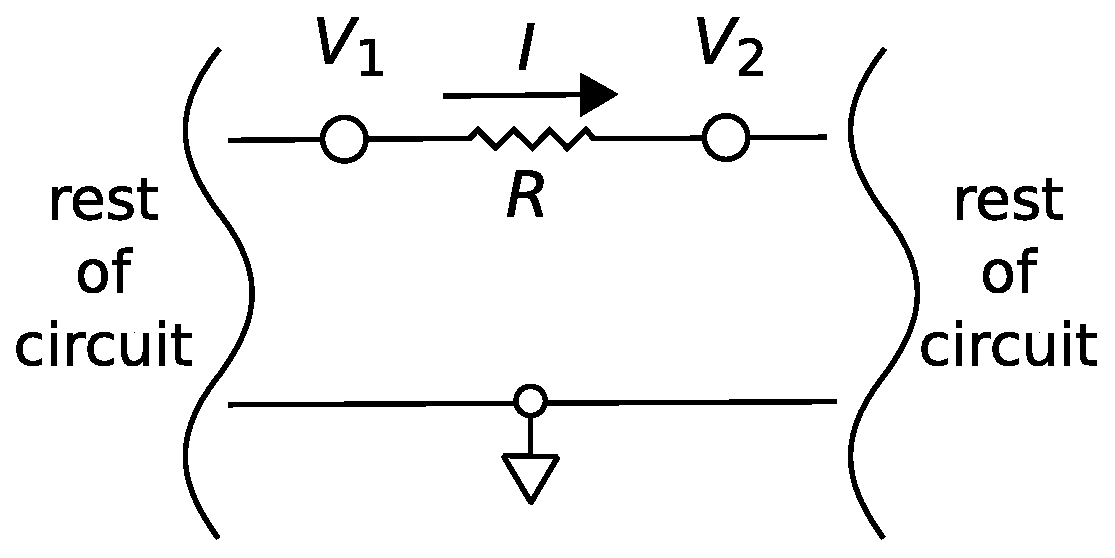
\includegraphics[width=2.5in]{modules/m0064_fResistor.eps}
% https://commons.wikimedia.org/wiki/File:M0064_fResistor.svg
}}{The diagram shows part of a circuit. Two curved lines on the left and right side of the figure indicate where the rest of the circuit is. The top branch has two nodes, labeled V sub 1 and V sub 2. Between them is a resistor (R), with an arrow pointed to the right to indicate the path of the current. On the bottom branch is a symbol for ground. }
\end{center} 
\centerline{\scriptsize 
\copyright~\hyperref[m0064_fResistor_Credit]{K.\ Kikkeri} 
\href{https://creativecommons.org/licenses/by-sa/4.0/}{CC BY~SA 4.0} 
} 
\caption{
\label{m0064_fResistor}
A resistor in a larger circuit, used as an example to demonstrate the concept of node voltages. 
}
\end{figure}

So, can we establish a datum in general electrostatic problems that works the same way?
The answer is yes.
The datum is arbitrarily chosen to be a sphere that encompasses the universe; i.e., a sphere with radius $\to\infty$.
Employing this choice of datum, we can use Equation~\ref{m0064_eV12} to define $V({\bf r})$, the potential at point ${\bf r}$, as follows:
%
\begin{equation}
\boxed{
V({\bf r}) \triangleq - \int_{\infty}^{{\bf r}} {\bf E} \cdot d{\bf l}
}
\label{m0064_eVP}
\end{equation}

%ORB HIGHLIGHT
\begin{mdframed}[backgroundcolor=yellow!20,nobreak=true] 
The electrical potential at a point, given by Equation~\ref{m0064_eVP}, is defined as the potential difference measured beginning at a sphere of infinite radius and ending at the point ${\bf r}$.  The potential obtained in this manner is with respect to the potential infinitely far away.
\end{mdframed}

In the particular case where ${\bf E}$ is due to the point charge at the origin:
%
\begin{equation}
V({\bf r}) = - \int_{\infty}^{{\bf r}} \left[ \hat{\bf r}\frac{q}{4\pi\epsilon r^2}  \right] \cdot d{\bf l}
\end{equation}
%
The principle of \emph{independence of path} (Section~\ref{m0062_Independence_of_Path}) asserts that the path of integration doesn't matter as long as the path begins at the datum at infinity and ends at ${\bf r}$. 
So, we should choose the easiest such path.
The radial symmetry of the problem indicates that the easiest path will be a line of constant $\theta$ and $\phi$, so we choose $d{\bf l}=\hat{\bf r}dr$.
Continuing:
%
\begin{flalign}
V({\bf r}) &= - \int_{\infty}^{r} \left[ \hat{\bf r}\frac{q}{4\pi\epsilon r^2}  \right] \cdot \left[ \hat{\bf r}dr \right] \\
           &= - \frac{q}{4\pi\epsilon} \int_{\infty}^{r} \frac{1}{r^2} dr \\
           &= + \frac{q}{4\pi\epsilon} \left.\frac{1}{r}\right|^{r}_{\infty} %= \left(-\frac{q}{4\pi\epsilon r}\right) - 0
\end{flalign}
%
so
%
\begin{equation}
\boxed{
V({\bf r}) = + \frac{q}{4\pi\epsilon r}
}
\label{m0064_eV}
\end{equation}
%
(Suggestion: Confirm that Equation~\ref{m0064_eV} is dimensionally correct.)
In the context of the circuit theory example above, this is the ``node voltage'' at ${\bf r}$ when the datum is defined to be the surface of a sphere at infinity.
Subsequently, we may calculate the potential difference from any point ${\bf r}_1$ to any other point ${\bf r}_2$ as
%
\begin{equation}
V_{21} = V({\bf r}_2)-V({\bf r}_1)
\end{equation}
%
and that will typically be a \emph{lot} easier than using Equation~\ref{m0064_eV12}.

It is not often that one deals with systems consisting of a single charged particle.
So, for the above technique to be truly useful, we need a straightforward way to determine the potential field $V({\bf r})$ for arbitrary distributions of charge.
The first step in developing a more general expression is to determine the result for a particle located at a point ${\bf r}'$ somewhere other than the origin.
Since Equation~\ref{m0064_eV} depends only on charge and the distance between the field point ${\bf r}$ and ${\bf r}'$, we have
%
\begin{equation}
V({\bf r};{\bf r}') \triangleq + \frac{q'}{4\pi\epsilon \left|{\bf r}-{\bf r}'\right|}
\label{m0064_eVd}
\end{equation}
%
where, for notational consistency, we use the symbol $q'$ to indicate the charge.
Now applying superposition, the potential field due to $N$ charges is
%
\begin{equation}
V({\bf r}) = \sum_{n=1}^N { V({\bf r};{\bf r}_n) }
\end{equation}
%
Substituting Equation~\ref{m0064_eVd} we obtain:
%
\begin{equation}
\boxed{
V({\bf r}) = \frac{1}{4\pi\epsilon} \sum_{n=1}^N { \frac{q_n}{\left|{\bf r}-{\bf r}_n\right|} }
}
\label{m0064_eVN}
\end{equation}
%
%ORB HIGHLIGHT
\begin{mdframed}[backgroundcolor=yellow!20,nobreak=true] 
Equation~\ref{m0064_eVN} gives the electric potential at a specified location due to a finite number of charged particles.
\end{mdframed}
%
The potential field due to continuous distributions of charge is addressed in Section~\ref{m0065_V_due_to_a_Continuous_Distribution_of_Charge}. 


